\chapter{Appendix}

\begin{subequations}
    \label{eq:Feature}
\begin{align}
    CN_A &= \sum_{B \neq A}^{N_\mathrm{atoms}} \dfrac{1}{1+\exp\left(\dfrac{-16a\cdot 4 (R_{A,\mathrm{cov}}+R_{B,\mathrm{cov}})}{3R_{AB}-1}\right)} \\
    CN^\mathrm{ext} &= \sum_{B \neq A}^{N_\mathrm{atoms}} \dfrac{CN_B}{f_\mathrm{damp}(R_A,R_B)}\\
    q_A &= Zg_A - \sum_{\mu \in A}^{N_\mathrm{BF}}\sum_{\nu}^{N_\mathrm{BF}} P_{\mu \nu} S_{\mu \nu}\\
    q_A^\mathrm{ext} &= q_A + \sum_{B \neq A}^{N_\mathrm{atoms}} \dfrac{q_B}{f_\mathrm{damp}}\\
    \mu_A^\alpha &= \sum_{l\in A} \sum_{\kappa \in l \in A} \sum_{\lambda} P_{\kappa \lambda}\left(\alpha_A S_{\lambda \kappa} - D_{\lambda \kappa}^{\alpha}\right)\\
    \mu_A^{\alpha,\mathrm{ext}} &= \mu_A^{\alpha} + \sum_{B \neq A} \dfrac{\mu_B^\alpha - \alpha_{AB} q_B}{f_\mathrm{damp} \cdot (CN_B + 1)}\\
    \mathrm{with}&:~\alpha_{AB} = \alpha_A - \alpha_B\\
    \mu_{A,p}^{\alpha,\mathrm{ext}} &= \mu_A^\alpha + \sum_{B \neq A} \dfrac{\mu_B^\alpha+ \alpha_{AB} p_B}{f_\mathrm{damp} (CN_B+1)}\\
    \theta_A^{\alpha \beta} &=   \sum_{l \in A} \dfrac{3}{2}\Theta_l^{\alpha \beta} - \dfrac{\delta^{\alpha \beta}}{2} (\Theta^{xx}_l + \Theta^{yy}_l +\Theta^{zz}_l) \\
    \mathrm{with}&:~\Theta_l^{\alpha \beta} = \sum_{\kappa \in l \in A} \sum_A P_{\kappa \lambda} \left(\alpha_A D_{\lambda \kappa}^\beta +\beta_A D_{\lambda \kappa}^\alpha - \alpha_A \beta_A S_{\lambda \kappa } - Q_{\lambda \kappa}^{\alpha \beta}\right) \nonumber \\
    \mathrm{and}&:~\delta^{\alpha \beta}=\begin{cases}
     1~\mathrm{if}: \alpha = \beta \\
     0~\mathrm{if}: \alpha \neq \beta\\   
    \end{cases} \nonumber \\
    \bm{\uptheta}_A &= \left(\begin{matrix}
        \theta_A^{\mathrm{xx}} & \theta_A^{\mathrm{xy}} & \theta_A^{\mathrm{xz}} \\
        \theta_A^{\mathrm{xy}} & \theta_A^{\mathrm{yy}} & \theta_A^{\mathrm{yz}} \\
        \theta_A^{\mathrm{xz}} & \theta_A^{\mathrm{yz}} & \theta_A^{\mathrm{yz}} \\
    \end{matrix}\right) \times \textbf{1}\\
    \theta_A^{\mathrm{ext},\alpha \beta} &= \theta_A^{\alpha \beta} + \dfrac{\theta^{\alpha \beta}_B + \delta \theta^{\alpha \beta}_B}{f_\mathrm{damp}(CN_B+1) }\\
    \bm{\uptheta}_A^\mathrm{ext} &= \left(\begin{matrix}
        \theta_A^{\mathrm{ext,xx}} & \theta_A^{\mathrm{ext,xy}} & \theta_A^{\mathrm{ext,xz}} \\
        \theta_A^{\mathrm{ext,xy}} & \theta_A^{\mathrm{ext,yy}} & \theta_A^{\mathrm{ext,yz}} \\
        \theta_A^{\mathrm{ext,xz}} & \theta_A^{\mathrm{ext,yz}} & \theta_A^{\mathrm{ext,yz}} \\
    \end{matrix}\right) \times \textbf{1}
\end{align}

\begin{align}
    E_{A,\mathrm{EHT}} &= \sum_{k \in A} \sum_k P_{k\lambda} H_{k\lambda}\\
    E_{A,\mathrm{rep}} &= \sum_{B \neq A}^{M} \dfrac{1}{2} \dfrac{Y_{A}^\mathrm{eff}Y_{B}^\mathrm{eff}}{R_{AB}}
    \cdot \exp \left(\alpha_A \alpha_B \right)^{0.5} R_{AB}^{k_\mathrm{rep}}\\
    E_{A,\mathrm{disp}}^{(2)} &= \sum_{A \neq B} \sum_{n=6,8} -s_n \dfrac{1}{2}
    \dfrac{C_n^{AB}(q_a,CN_\mathrm{cov}^A,q_b,CN_\mathrm{cov}^B)}{R_{AB}^n} f_{n}^\mathrm{damp,BJ}(R_{AB})\\
    E_{A,\mathrm{disp}}^{(3)} &= \sum_{B \neq A} \sum_{C \neq B \neq A} 
    -s_9 \dfrac{1}{3} 
    \dfrac{(3 \cos(\theta_{ABC}) \cos(\theta_{BCA} \cos(\theta_{CBA}) + 1))}{(R_{AB}R_{AC}R_{BC})^3} \nonumber\\ 
    &\cdot  C_9^{ABC}(CN_\mathrm{cov}^A,CN_\mathrm{cov}^B,CN_\mathrm{cov}^C) \cdot 
    f_{9}^\mathrm{damp,zero}(R_{AB},R_{AC},R_{BC})\\
    E_{A,\mathrm{AES}} &= E_{A,q\mu} + E_{A,q\theta} + E_{A,\mu\mu} \nonumber \\
    &= \sum_{B \neq A} \dfrac{1}{2} \bigg(f_3(R_{AB})\big[q_A(\bm{\mu}_B^\intercal\textbf{R}_{BA}) + q_B (\bm{\upmu}_A^\intercal)\textbf{R}_{AB} \big] \nonumber\\
    &+ f_5(R_{AB}) \big[q_A\bm{R}_{BA}^\intercal \bm{\Uptheta}_B \bm{R}_{BA} +q_B\bm{R}_{BA}^\intercal \bm{\Uptheta}_A \bm{R}_{BA} \nonumber \\
    &- 3 (\bm{\upmu}_A^\intercal\bm{R}_{AB})(\bm{\upmu}_B^\intercal\bm{R}_{AB}) +  (\bm{\upmu}_A^\intercal \bm{\upmu}_B R_{AB}^2)  \big] \bigg)\\
    E_{A,\mathrm{AXS}} &= \left( f_\mathrm{XC}^{\mu_A}|\bm{\upmu}_A|^2  + f_\mathrm{XC}^{\Theta_A}||\bm{\Uptheta}_A||^2  \right) \\
    E_{A,\mathrm{IES+IXC}} &= \dfrac{1}{2} \sum_{B \neq A} \sum_{l \in A} \sum_{l' \in B} q_{A,l} q_{B,l'} \gamma_{AB,ll'} + \dfrac{1}{3} \sum_{l \in A} \Gamma_{A,l} q_{A,l}^3
\end{align}
\end{subequations}

\begin{table}[H]
    \centering
    \caption[List of indices used for the differentiation of Hessian elements.]{Indices used for the different elements in a Hessian matrix block to differ between the elements.}
        \begin{tabular}{c c c c | c }
            \hline
            & &  Indexed& & Permuted \\
            Hessian element &  $x^\mathrm{idx}$ & $y^\mathrm{idx}$ & $z^\mathrm{idx}$ & Index\\
            \hline
            \\[-1em]
            $\dfrac{\partial^2 E}{\partial x_A \partial x_B}$ & 2 & 0 & 0 & 0\\
            \\[-1em]
            $\dfrac{\partial^2 E}{\partial x_A \partial y_B}$ & 1 & -1 &  0 & 1\\
            \\[-1em] 
            $\dfrac{\partial^2 E}{\partial x_A \partial z_B}$ & 1 & 0 &  -1 & 2\\
            \\[-1em]
            $\dfrac{\partial^2 E}{\partial y_A \partial x_B}$ & -1 & 1 &  0 & 1\\
            \\[-1em]
            $\dfrac{\partial^2 E}{\partial y_A \partial y_B}$ & 0 & 2 &  0 & 0\\
            \\[-1em]
            $\dfrac{\partial^2 E}{\partial y_A \partial z_B}$ & 0 & 1 &  -1 & 2\\
            \\[-1em]
            $\dfrac{\partial^2 E}{\partial z_A \partial x_B}$ & -1 & 0 &  1 & 2\\
            \\[-1em]
            $\dfrac{\partial^2 E}{\partial z_A \partial y_B}$ & 0 & -1 &  1 & 2\\
            \\[-1em]
            $\dfrac{\partial^2 E}{\partial z_A \partial z_B}$ & 0 & 0 &  2 & 3\\
            \\[-1em]
            \hline 
        \end{tabular}
    \label{tab:Indices}
\end{table}

\begin{table}[H]
    \centering
    \caption[]{Permutation of the coordinates for each Hessian element.
    At first the permutation of the vectors is shown.
    After that, the change of the elements of a matrix, for example, for the quadrupole moment is shown.}
        \begin{tabular}{c c c c c c c c c c}
            \hline\\[-1em]
            Hessian &\\
            &$\dfrac{\partial^2 E}{\partial x_A \partial x_A}$ & $\dfrac{\partial^2 E}{\partial x_A \partial y_A}$ &
            $\dfrac{\partial^2 E}{\partial x_A \partial z_A}$ &$\dfrac{\partial^2 E}{\partial y_A \partial x_A}$ &
            $\dfrac{\partial^2 E}{\partial y_A \partial y_A}$ &$\dfrac{\partial^2 E}{\partial y_A \partial z_A}$ &
            $\dfrac{\partial^2 E}{\partial z_A \partial x_A}$ & $\dfrac{\partial^2 E}{\partial z_A \partial y_A}$ &
            $\dfrac{\partial^2 E}{\partial z_A \partial z_A}$ \\[+0.7em]
            \hline
            Vector\\
            x &  x  &  y    & z  & x   &y   & z     &x     & y  & z\\ 
            y &  y  &  x    & x  & y   & z  & y     & z    & z  & x \\
            z &  z  & $-$z  & y  & z   &x   &$-$x   & $-$y & x  & y\\
            \hline 
            Matrix\\
            xx & xx & yy    & zz & xx  & yy & zz    & xx   & yy & zz \\
            yy & xy & xx    & xx & yy  & zz & yy    & zz   & zz & xx \\
            zz & xz & zz    & yy & zz  & xx & xx    & yy   & xx & yy \\
            xy & xy & xy    & xz & xy  & yz & yz    & xz   & yz & xz \\
            xz & xz & $-$yz & yz & xz  & xy & $-$xz & $-$xy& xy & yz \\
            yz & yz & $-$xz & xy & yz  & xz & $-$xy & $-$yz& xz & xy \\
            \hline 
        \end{tabular}
    \label{tab:Permutation}
\end{table}


\begin{figure}[H]
    \hspace*{-0.25cm}
    \subfloat[homonuclear model]
    {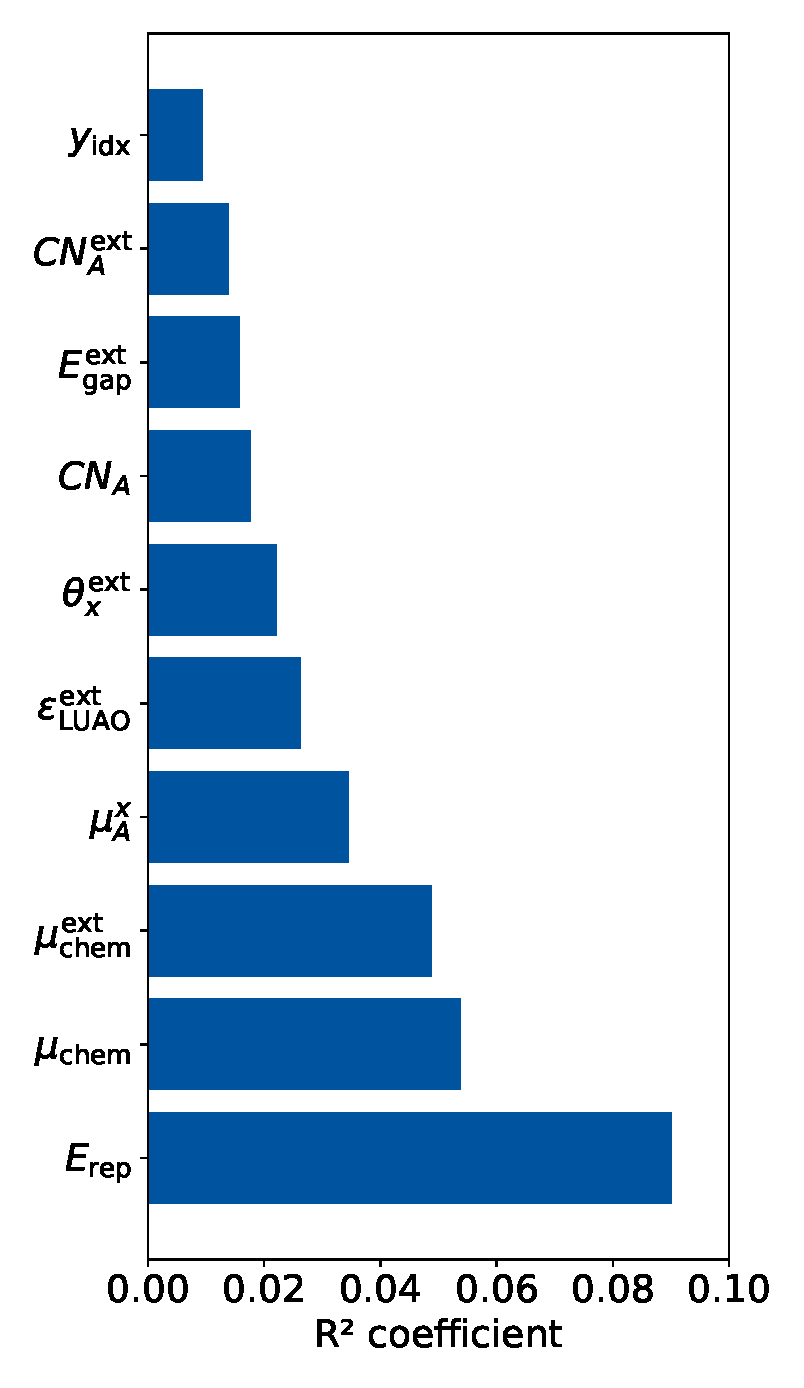
\includegraphics[width = 0.48\textwidth]{PearsonCorrelationCoeffiecient/PCC_diag_perm.eps}}
    \hspace*{0.25cm}
    \subfloat[heteronuclear model]{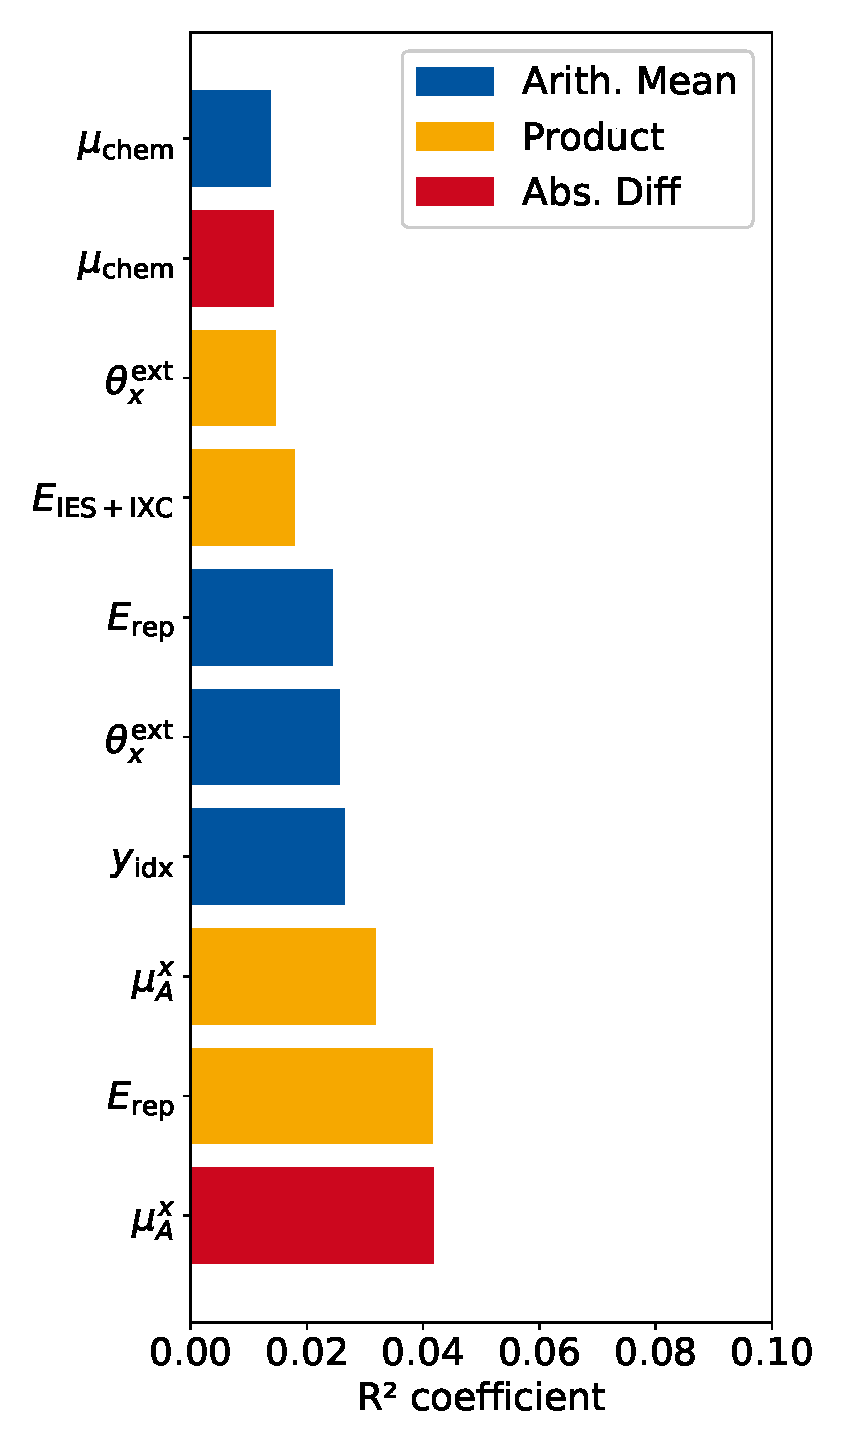
\includegraphics[width = 0.48\textwidth]{PearsonCorrelationCoeffiecient/PCC_ndiag_perm.eps}}
    \caption[Pearson Correlation Coefficient for the ten most important features (Gen--Perm model).]{
                Pearson Correlation Coefficient for the features used for the homonuclear and heteronuclear model.
                The ten features with the highest coefficients are shown for each model.
                The features are constructed with the Gen--Perm model.
                }
    \label{fig:PCC_perm}
\end{figure}

\begin{figure}[H]
    \hspace*{-0.25cm}
    \subfloat[homonuclear model]
    {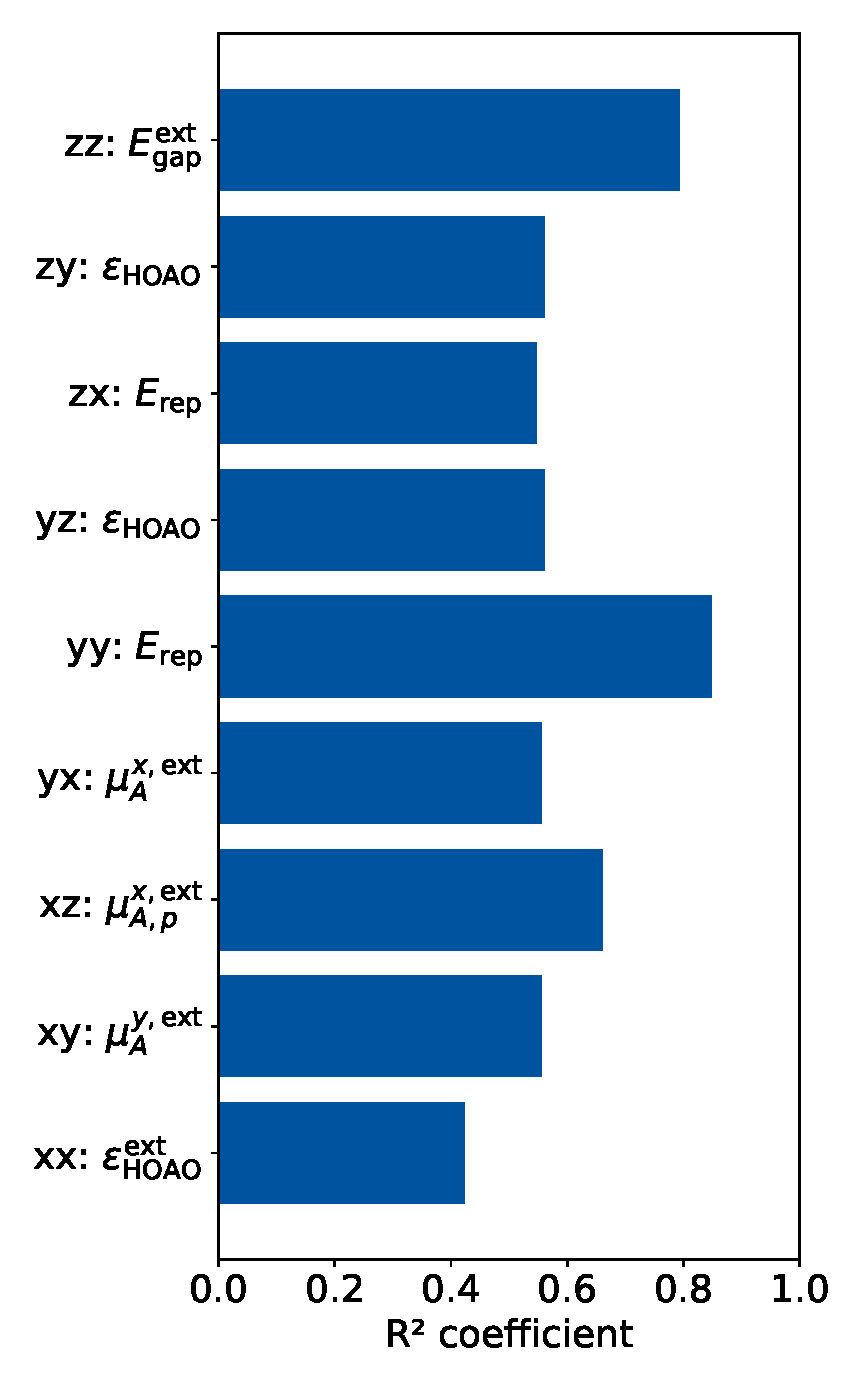
\includegraphics[width = 0.48\textwidth]{PearsonCorrelationCoeffiecient/PCC_element_specific_diag_perm.eps}}
    \hspace*{0.25cm}
    \subfloat[heteronuclear model]{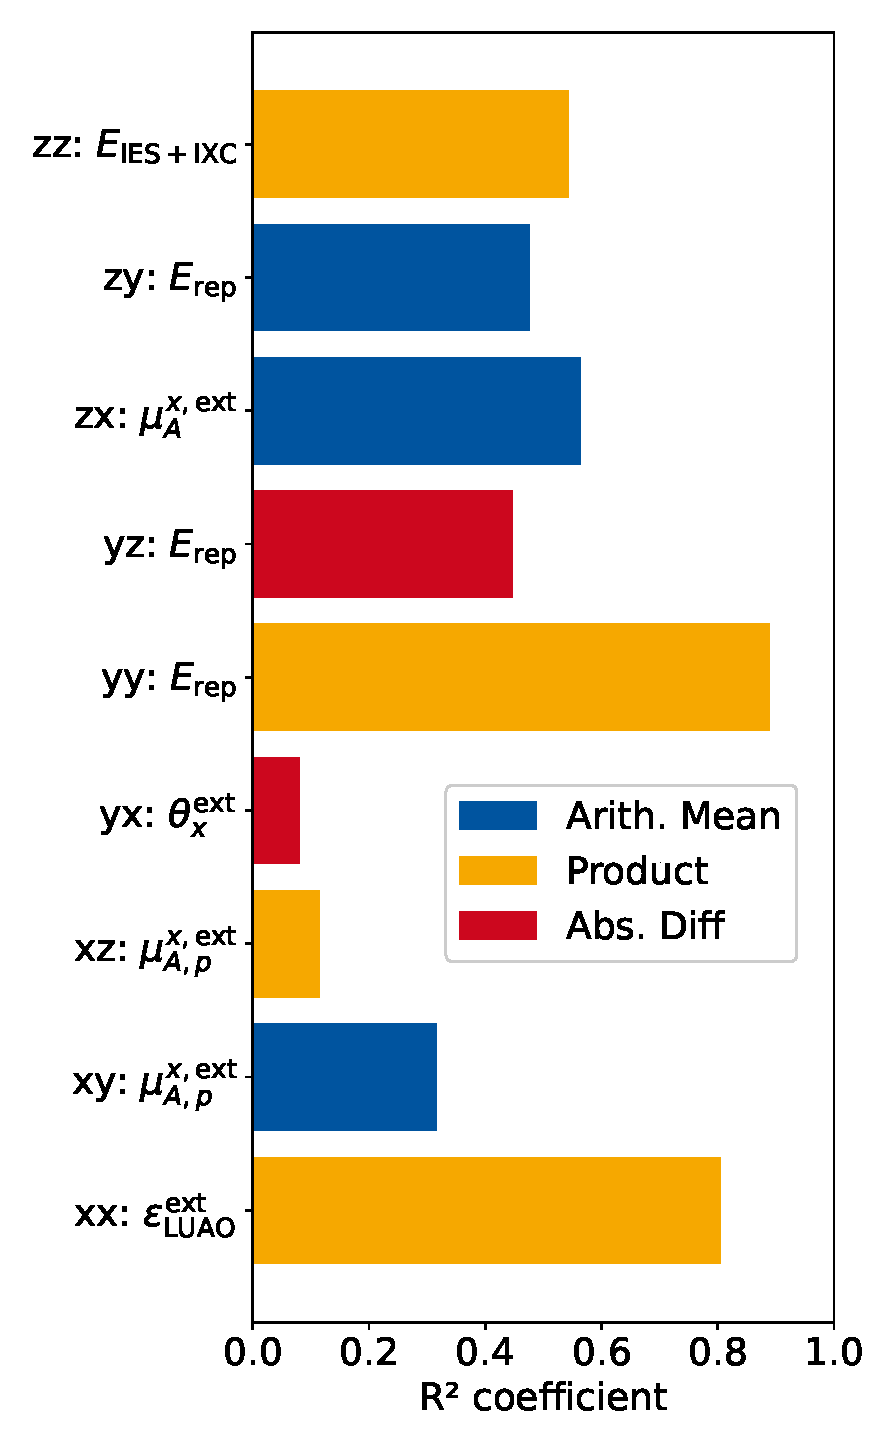
\includegraphics[width = 0.48\textwidth]{PearsonCorrelationCoeffiecient/PCC_element_specific_nondiag_perm.eps}}
    \caption[Best Pearson Correlation Coefficient computed element wise (Gen--Perm model).]{
        Highest Pearson Correlation Coefficient specifically computed for each Hessian element for the homo-- and heteronuclear model.
        The abbreviation ab corresponds to the elements $\frac{\partial^2 E}{\partial a_A \partial b_B}$.
        The features are constructed with the Gen--Perm model.
                }
    \label{fig:PCC_elementwise_Perm}
\end{figure}

\begin{figure}[H]
    \centering
    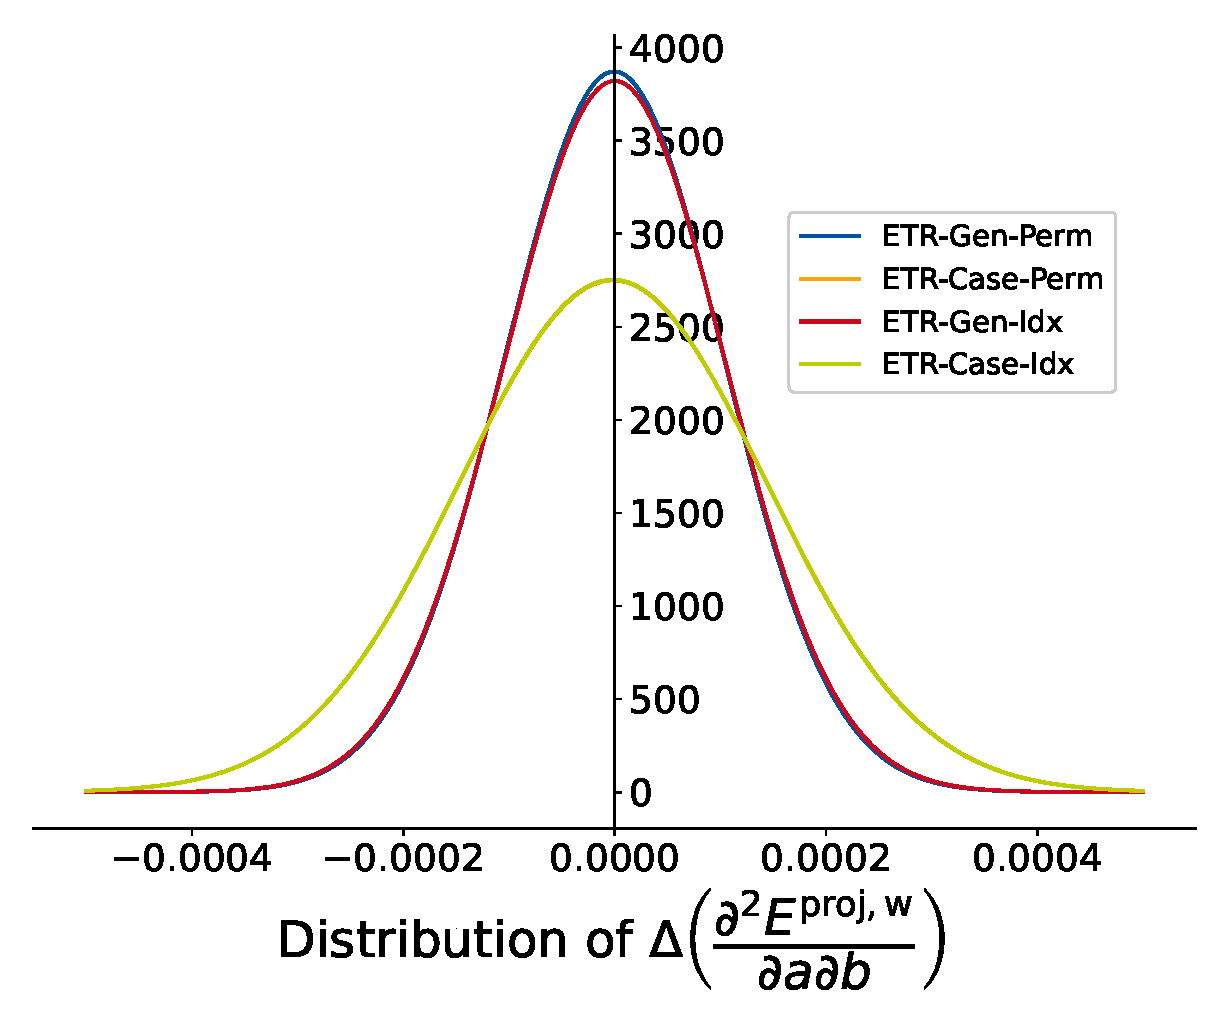
\includegraphics[width = \textwidth]{ErrorDistGraphs/error_distribution_ml_hess_w.eps}
    \caption[Gaussian type distribution for the prediction of weighted projected Hessian elements.]{
    Distribution of $\Delta \left(\frac{\partial^2 E^\mathrm{proj,w}}{\partial a \partial b}\right)$ for different models.
    In every model, the ETR was used.
    A Gaussian distribution is assumed.
    For this the median and standard deviation of $\Delta \left(\frac{\partial^2 E^\mathrm{proj,w}}{\partial a \partial b}\right)$ are computed. }    \label{fig:ErrorDistHessW}
\end{figure}

\begin{figure}[H]
    \centering
    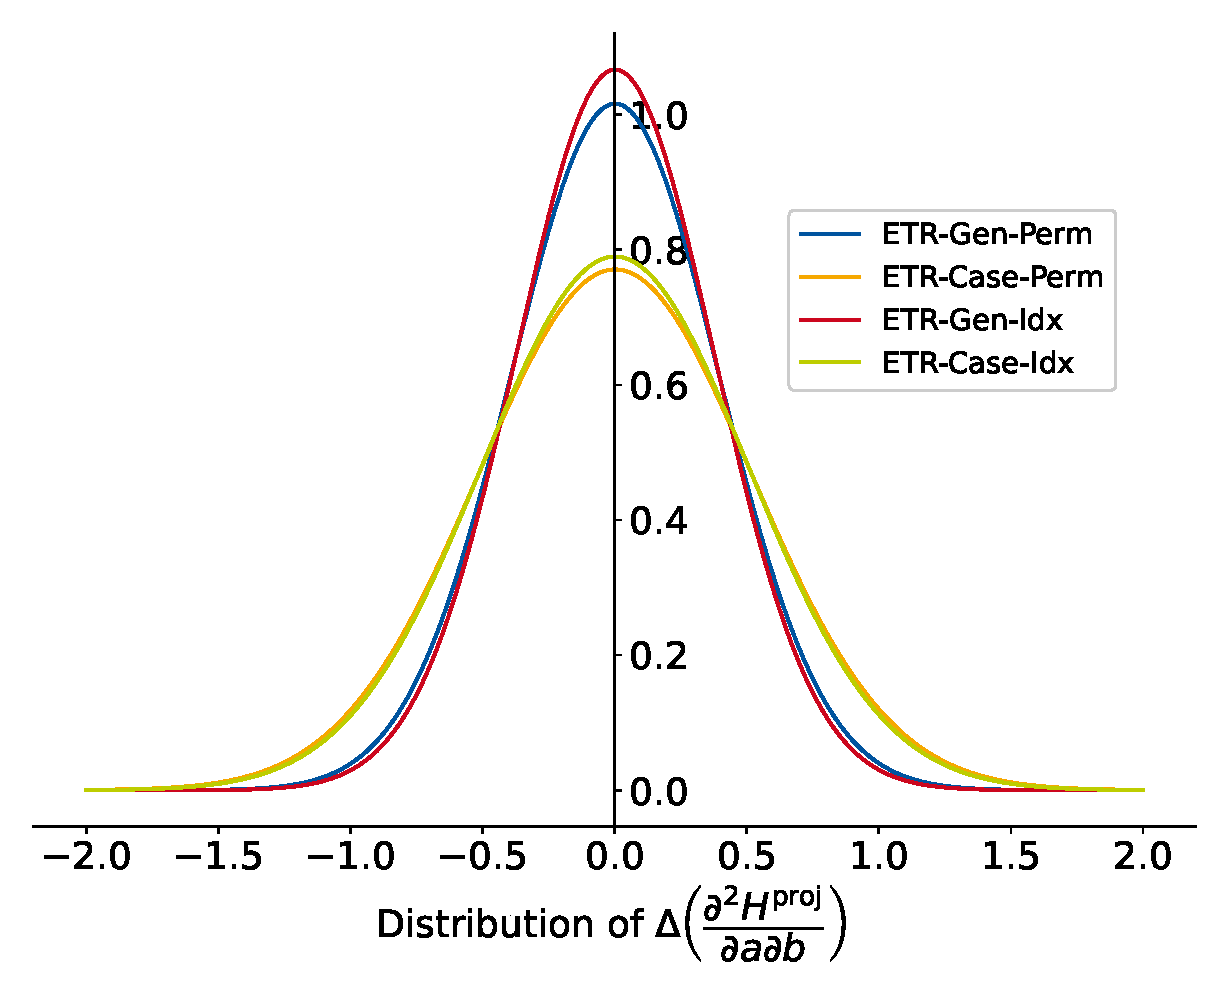
\includegraphics[width = \textwidth]{ErrorDistGraphs/error_distribution_ml_hess_p.eps}
    \caption[Gaussian type distribution for the prediction of projected Hessian elements.]{
    Distribution of $\Delta \left(\frac{\partial^2 E^\mathrm{proj}}{\partial a \partial b}\right)$ for different models.
    In every model, the ETR was used.
    A Gaussian distribution is assumed.
    For this the median and standard deviation of $\Delta \left(\frac{\partial^2 E^\mathrm{proj}}{\partial a \partial b}\right)$ are computed. }
    \label{fig:ErrorDistHessP}
\end{figure}
    
\begin{figure}[H]
    \centering
    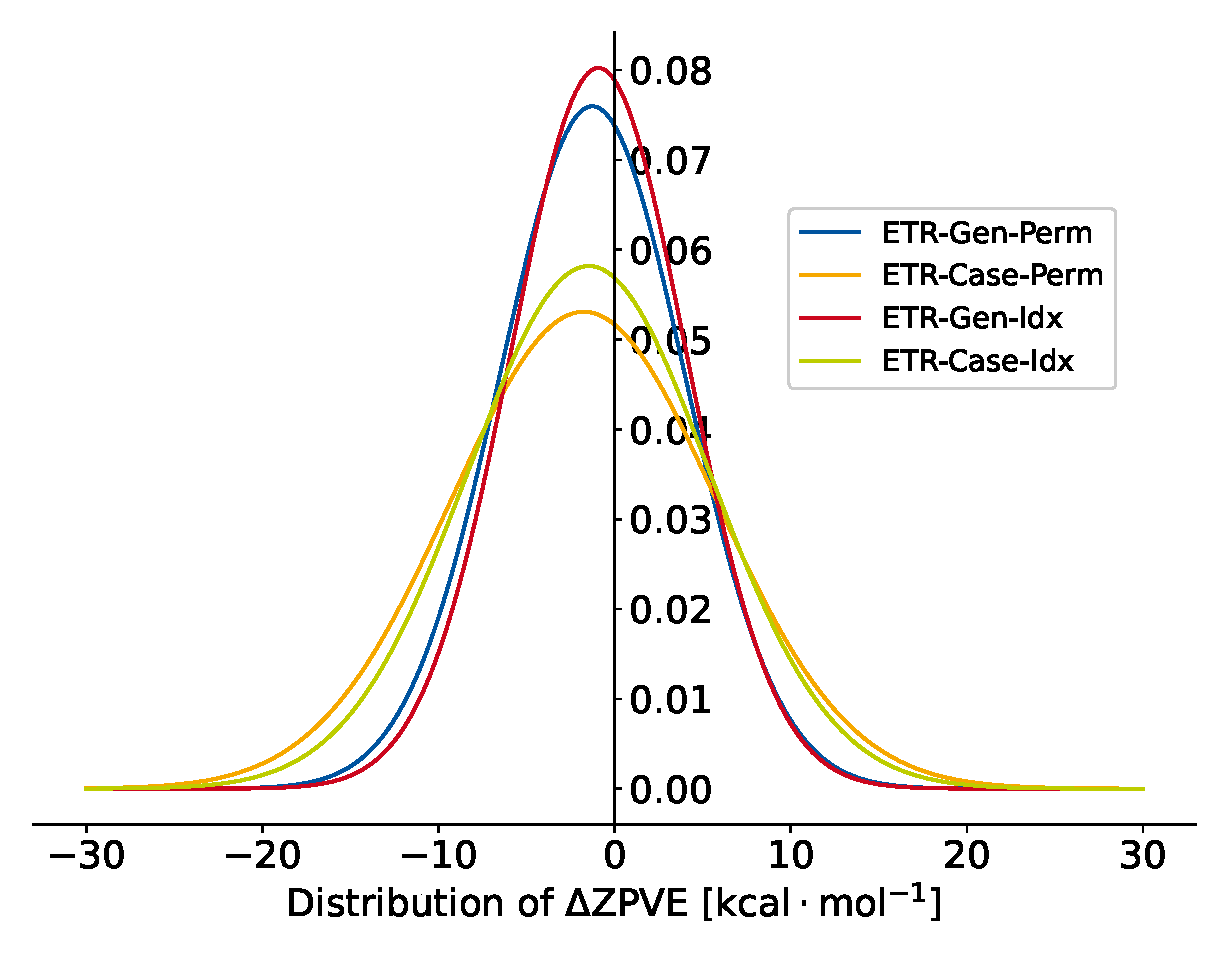
\includegraphics[width = \textwidth]{ErrorDistGraphs/error_distribution_ml_ZPE.eps}
    \caption[Gaussian type distribution for the prediction of zero point energy.]
    {Distribution of $\Delta \mathrm{ZPE}$ for different models.
    In every model, the ETR was used.
    A Gaussian distribution is assumed.
    For this the median and standard deviation of $\Delta \mathrm{ZPE}$ are computed.}
    \label{fig:ErrorDistZPE}
\end{figure}
